%!TEX root =  main.tex

\section{Introduction}
When we find evidence for a hypothesis that we have held in the back of our minds, our belief in that hypothesis increases. This is the essence of reasoning with evidence. Our goal in reasoning with evidence is to find a method that will lead us to believe as many true hypotheses as we can, given the evidence that we have.

However, the relationship between evidence and hypotheses is elusive. How can we be sure that some evidence supports some hypothesis? Even if we know that it does, how can we express how strong the piece of evidence is? Some evidence is very weak, and only after a tedious process of ruling out other factors and careful investigation and collection of other pieces of evidence, we can come to a conclusion about a hypothesis. On the other hand, some evidence is so strong that it leaves no room for doubt.

We can consider three main approaches for reasoning about hypotheses using evidence within the domain of AI and Law \citep{diBelloVerheij2018}: an argumentative, a scenario-based, and a probabilistic approach. One subfield of the probabilistic approach is the use of Bayesian Networks. Bayesian Networks can make explicit how our beliefs about events should change given that we find certain pieces of evidence for them. This idea of correctly updating on new information make BNs an interesting tool in the courtroom. A Bayesian Network might make transparent how reasoners should update their beliefs based on the evidence, which might increase transparency and fairness. In the ideal case, a Bayesian Network might stop a judge from making a reasoning error.

However, creating and using BNs is far from straightforward for both the builder and the interpreter. From \citet{deKoeijer2020}: it is complex, time-consuming, hard to explain, and, the ``repeatability [...] leaves much to be desired. Node definitions and model structures are often directed by personal habits, resulting in different models for the same problem, depending on the expert''. This subjectivity is pervasive throughout the Bayesian Network: the events selected, arcs drawn, and numbers elicited are subjective and seem empirically untestable in the data-poor environment of AI and law. These problems might be mitigated in part by evaluation criteria. 

These evaluation criteria, however, do do not always sufficiently safeguard against an incorrect network, which is a network that predict the `wrong' outcome based on some set of evidence. One example of this is seen in Figure~\ref{love}, which is a network taken from \citet{vanLeeuwen2019}. This network is unfairly biased towards the scenario that the suspect is guilty. In the original paper, we entered the evidence that was found during the trial, and the response of the network seemed sensible. However, in that same network, we are now entering a different evidence: there is no body, no signs of violence, no car with bloodstains, no evidence of existing conflict. The only evidence that the prosecution has, are some phone calls, and  testimony of the suspect about amnesia that does not match medical reality. The outcome of the network is that the suspect is guilty (scn1 is `yes'). But the evidence that is entered into this network, would not reasonably support this conclusion. No reasonable arguer would argue that this state of evidence is sufficient for a guilty verdict.

\begin{figure}[htbp]
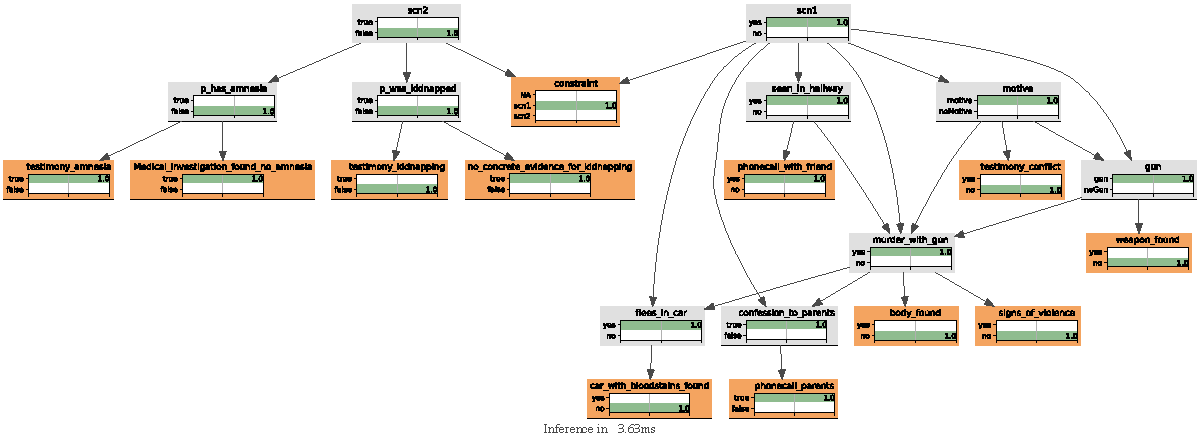
\includegraphics[width=\linewidth]{images/oldnetwork.pdf}
\caption{Example of subjective probability estimation resulting in a guilty verdict for insufficient evidence}
\label{love}
\end{figure}%


The cause of the bias of this BN towards the guilty verdict is due to the modeller's inability to rationally consider all possible evidence states. The aim of this project is to define a method for the modeller to evaluate the BN over all possible evidence states, by grounding the BN in an agent-simulation of a crime. We can model crime cases using simulations to a level of realism we desire, measure the frequencies of events that emerge out of this simulation by running the simulation multiple times. In the agent-based system, we have full control over and full knowledge of the world that we are reasoning about, hence we can create a grounding that can be used to evaluate the BN. We can test whether our method of evaluating all possible evidence states works by comparing the predicted output of the BN with the frequency information about the output from the simulation. Then, we will discuss whether it is plausible that this method of evaluation generalises to real life\footnote{The simulation can be interacted with at \url{https://shielded-journey-34533.herokuapp.com} \\ Code for this project can be found at \url{https://github.com/aludi/simulationTest}}.


\section{Background}

% reasoning with evidence
%Ook kort bespreken/benoemen: Di Bello and Verheij (2018) discuss how central analytic goals can be handled using each of the approaches.
We want to create grounded Bayesian Networks for reasoning with evidence. This can be done by creating a agent-based simulation, building BNs based on the events in this simulation, and testing the evaluation method on that BN. In this section, the relevant background is laid out on reasoning with evidence, Bayesian Networks, existing evaluation methods for BNs, and agent-based simulations.


\subsection{Reasoning with evidence}
We consider three main directions in the field of reasoning with evidence within law \citep{Verheij2015}, \citep{diBelloVerheij2018}. 

The first direction is via argumentation approaches, where hypotheses and evidence are represented as propositions that attack or support each other, as originating in \citep{wigmore1931} and in part unified by \citet{dung1995} \citep{benchcapon2019}. An example of an implementation of an argumentation framework in AI and law is ASPIC+ \citep{prakkenEtal2013}. 

The second direction is via scenario approaches, where more-or-less coherent hypotheses are combined into stories \citep{penningtonHastie1993}, \citep{wagenaar1993}, which are supported with evidence. Different types of stories need different pieces of evidence to be considered `valid' or `anchored' stories, and the extent to which different stories are anchored in the evidence determines how we assess them. 

The third direction is via probabilistic approaches, where hypotheses and evidence are assigned probabilities and the relation between hypothesis and evidence is represented with conditional probability, either by applying Bayes Law directly \citep{dahlman2020}, or by using Bayesian Networks. Bayesian Networks can represent aspects of a criminal case or can attempt a scenario-like hybrid and represent the entire case - modelling actual crime cases \citep{kadaneSchum1996}, \citep{Fenton2019},  cases from fiction \citep{Fenton2012} or fictionalised crime cases \citep{vanLeeuwen2019}. The BN can also represent specific (forensic) aspects of a case, like DNA or blood-spatter evidence, for methods see \citep{Meester2021}. Bayesian Networks can also integrate aspects of argumentation \citep{wieten2019}, \citep{timmer2016}, or of scenario-based construction \citep{vlek2016}.



\subsection{Bayesian Networks}

A Bayesian Network (BN) is a directed, acyclic graph that represents the joint probability distribution over a set of events \citep{pearl1988b}. BNs consists of nodes, arcs and conditional probability tables. A node is a random variable that represents an events. An arc represent a conditional relationships between two events, linking two nodes together. The two nodes are the parent and the child node, the probabilities in the child node are conditioned on the value that the parent node takes. The specification of these conditional probabilities is done in the conditional probability tables (CPT) of each node.

We show an example BN in Figure~\ref{exampleBN}. This is the basic form of the evidence idiom \citep{Fenton2012}: we have a cause as a parent node, and a consequence as a child node. In this context, we want to interpret the parent node as a `hypothesis', that we want to prove, but cannot observe directly. The child node is a piece of evidence that we can observe: it is either true, or false. Specifically instantiated, like in Figure~\ref{exampleBN}, we create a basic scenario: `suspect shot victim with gun' as the parent (hypothesis) node, and `bullet casings found on ground' as the child (evidence) node. We can use this network, with the probabilities as defined in the CPTs, to reason about the hypothesis given the evidence that we find.
 
In Figure~\ref{exampleBN}, the node `suspect shot victim with gun' is a hypothesis. Nodes with one or more incoming arcs are conditionally dependent on their parent node(s). In our example network, the node `bullet casings found on the ground' is conditionally dependent on its parent. The links between the nodes are links of conditional probability, and do not correspond to real-world causality, although they are sometimes interpreted as being causal \citep{Dawid2008}.

\begin{figure}[htbp]
\begin{center}
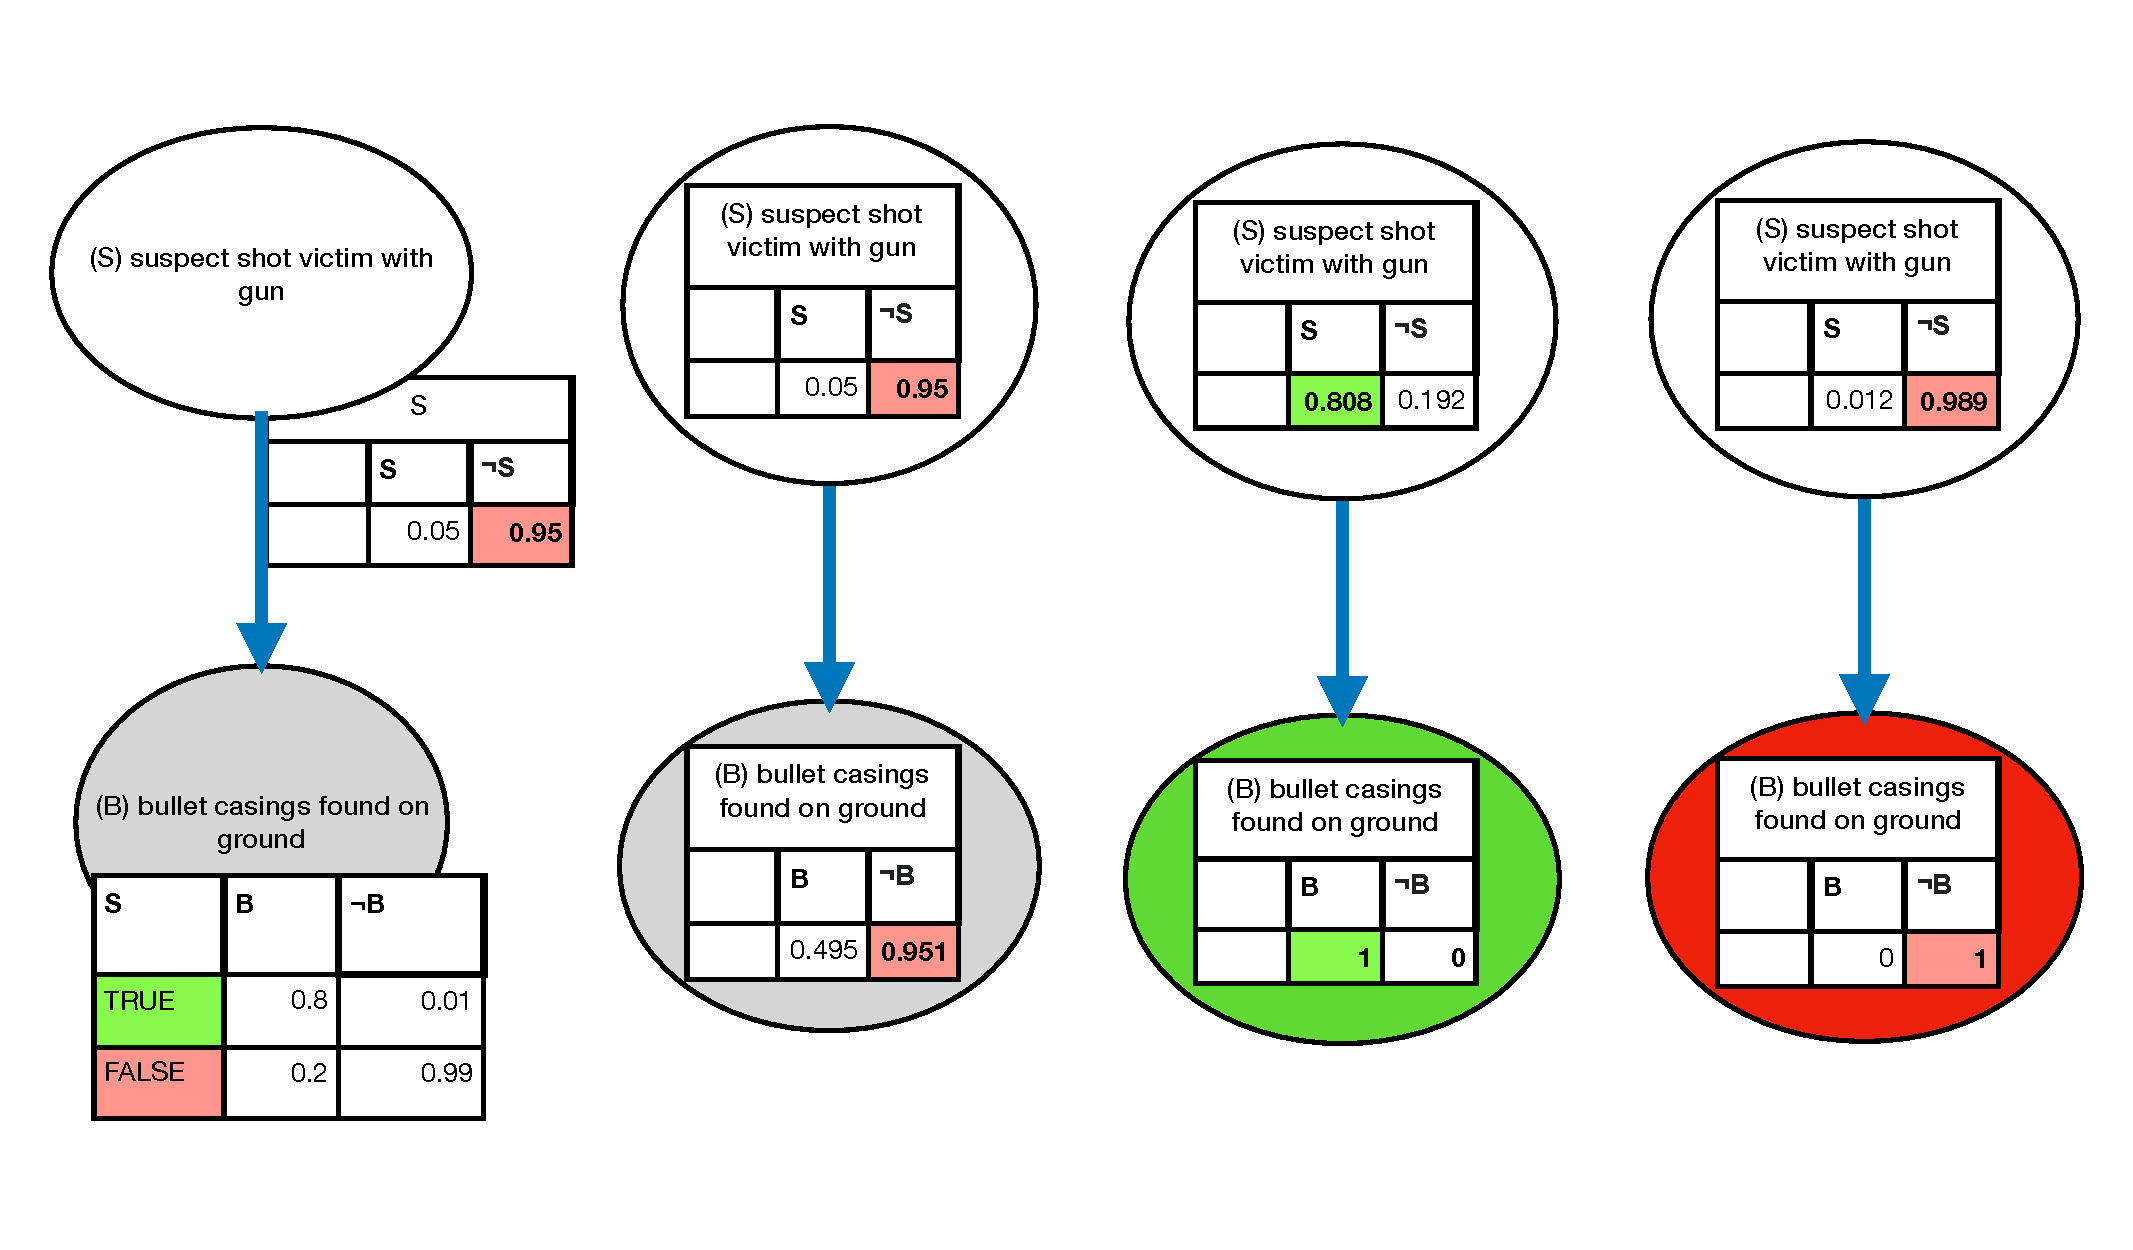
\includegraphics[width=\linewidth]{images/basicBayes}
\caption{Inference with Bayesian Networks: Defining the network with CPTS, entering no evidence, entering positive evidence, and entering negative evidence}
\label{exampleBN}
\end{center}
\end{figure}

The arcs and the CPTs tell us how we should reason about the hypothesis, given that we find some piece of evidence. This is done using Bayes Law.

\[ P(H | E) =  \frac{P(E | H) \cdot P(H)}{P(E)}\]


To apply this to our network let us say that we found $B$, so there are bullet casings on the ground. We want to know what this new evidence will do to our belief in $S$. This means that we are updating our belief in $S$, or finding the posterior of $S$, based on the evidence that we found $B$.

\[ P(S | B) =  \frac{P(B | S) \cdot P(S)}{P(B)}\]
\[ P(B | S) = 0.8, P(S) = 0.05, P(B) = 0.8 \cdot 0.05 + 0.01 \cdot 0.95\]
\[ P(S | B) =  \frac{0.8 \cdot 0.05}{0.8 \cdot 0.05 + 0.01 \cdot 0.95} = 0.808\]

So now we have found the posterior of $S$, our belief in $S$ has increased from its prior probability of $0.05$, to its posterior probability of $0.808$, given evidence $B$. On the other hand, if we do not find bullet casings on the ground, our belief that the suspect shot the victim decreases from 00.5 to 0.012. 

Hence, we can exactly specify how our belief in a hypothetical event changes given all possible values of the evidence.This is the simplest form of Bayesian reasoning, with one piece of evidence, and one hypothesis. However, real life is not so simple: we are constantly reasoning with many pieces of evidence that might be conditioned on more than one parent node, resulting in tedious and error-prone calculations. This is where Bayesian Networks are useful. 

We can outsource the Bayesian calculation to the BN, however, the network itself has to be constructed in some way. This can be done by hand by modellers, in (proprietary) software with a GUI like AgenaRisk or Hugin. They can also be built, by hand, or automatically constructed from datasets in PyAgrum, \citep{pyagrum2020}, a free Python software package. In this project, PyAgrum was used.

\subsubsection{Evaluating Bayesian Networks}

There is a precedent for building Bayesian Networks to model reasoning with evidence in criminal cases, although these methods have not been used in court. However, even though there are methods for building BNs, it is unclear how we should validate and evaluate them. 

In data-rich domains, we can train Bayesian Networks on large amounts of frequency data and estimate the accuracy of the BN by cross-validation. We define a training set and a test set of the data (usually a 80/20 split). We construct the network based on the training data, 80\% of the input. Then, we test if the network learned the correct conditional probability relations on the final 20\% of the data, by comparing the expected output in the test data to the predicted output from the BN \citep{chen2012}. The 80/20 split allows us to know if the network is performing well on the entire dataset, and not just overfitting on the data that it has access to.

However, this approach towards BN validity through accuracy is implausible in BNs for court cases. The court cases involve one-of-a-kind events \citep{schum1982}, which means that it is unlikely that we can find frequency data on most of the nodes present in our BNs. This means that we cannot do an 80/20 type split in our data, as we only have one piece of data, which is the court case that we are modelling. This is why the probabilities in the BNs for court cases not pure frequencies, but instead subjective probabilities based on estimated frequencies, either elicited from experts or estimated by the modeller.

There are other ways of evaluating BNs than accuracy. The evaluation methods found in \citet{Fenton2019} and \citet{vlek2016}, who both model BNs based on real case studies, confine themselves to two approaches:

\begin{enumerate}

\item \textbf{Sensitivity analysis}

Sensitivity analysis tests the effect of small parameter changes in the CPTs of nodes on the outcome of the network. This is useful if the outcome of the network hinges on elicited or subjectively estimated probabilities. A sensitivity value of near 0 means that at the point of the CPT, a `small' change in the parameter would result in an infinitesimally small change in the output probability - this means that the CPT is not sensitive at all and a misestimation might not matter so much. However, a large sensitivity value means that the value is very sensitive to change - a small change in CPT might result in a meaningfully different output.  Since Bayesian Networks have many parameters per node, it is not trivial to perform a sensitivity analysis that takes into account all the nodes in the network, and interpret the results in a meaningful way - this would be an $n$-way sensitivity analysis \citep{gaag2007}.  

In \citet{vlek2016}, sensitivity analysis is mentioned, but not applied. On the other hand, in \citet{Fenton2019}, each individual hypothesis node is subjected to sensitivity analysis, to find out for how each of the parameters in the nodes need to change in order to result in a 0.95 or a 0.99 posterior for guilt. There are only a few ways that individual nodes can change that would result in a high probability of guilt, which means that the constructed BN is robust to small inaccuracies in subjectively elicited CPTs. However, in the paper, this is only shown for one evidence state. It is not clear how the BN would respond to `counterfactual' pieces of evidence.


\item \textbf{Cumulative evidence}

Another way of evaluating the response of the BN, is by seeing its response to cumulatively setting evidence. This way, we can see how much each piece of evidence (from the defence or the prosecution) changes our belief in the posterior of the output node(s). We could subjectively assess if it makes sense that a certain piece of evidence has a large, or small, effect on the posterior. In both \citep{Fenton2019} and \citep{vlek2016} this cumulative approach shows that, in general, the evidence from the defence decreases our belief that the suspect is guilty, and evidence from the prosecution increases our belief that the suspect is guilty. However, in both cases, the BN is only evaluated on one state of evidence. Both cases only test the cumulative probability of the output node by turning the evidence nodes to values that correspond to the findings of the court. However, this is a risky move, since this might lead to overfitting the probabilities in the CPTs, so that the network seems to reflect the right `evidence strength' on the court-found state of evidence, but is actually misrepresenting other combinations of evidence, without a way of checking if this is the case.




\end{enumerate}


Our findings in Figure~\ref{love} show that it is necessary to consider all possible combinations of evidence. If we have tunnel vision and only focus on the state of evidence that is found in court, we might create a network that overfits on one state of evidence. This means that if there was a re-trial and the court would decide that some pieces of evidence are not admissible after all, the BNs might show the unreasonable behaviour. Additionally, if we are building the BN before or during the court case, we cannot know yet which state we are in, as none of the evidence has been established yet. Therefore, the network should work correctly over all possible evidence states. If we want to take the premise behind BNs seriously, we have to create a network that gives sensible results for all possible combinations of evidence, not just the valuation of the evidence that is initially established in court.

\subsection{Simulation}

We are using agent-based simulations to investigate methods for evaluating Bayesian Networks. Agent-based modelling is a modelling primitive that allows researchers to study models in which agents interact with their environment and with other agents\citep{gilbert2000}. 

Agent-based modelling is useful for simulating criminal behaviour in spatially explicit ways. The actions of a thief and victim are constrained by geography and local knowledge (a thief can't move through buildings like a ghost, or steal from someone they have not seen). Due to specific interactions that arise out of the circumstances in each run of the simulation, we can collect frequency information about all the relevant events in our modelled scenario that would be hard to estimate with subjective probabilities or with mathematical (non-spatially explicit) models. Since we have full knowledge of the frequency of events in the simulation, we can use it as a `grounding', or baseline. In a sense, the simulation is a data-generating environment for criminal cases. If we look at the taxonomy of agent-based model levels in \citep{gilbert2005}, where level 3 is a simulation that really reflects the real world, and level 0 is a `caricature of reality, as established with simple graphical devices', the simulation in this paper is definitely at level 0, to reduce complexity. In this project, the simulations will be programmed in Python using the MESA framework  \citep{mesa2020}.

\section{Method}

Our goal is to establish a method for evaluating BNs by preventing overfitting on one evidence state. We can consider an approach in four stages.

\begin{enumerate}
\item We need a set of alternative scenarios that are to be modelled. These scenarios are written description of crime scenarios that contain the hypothetical events and evidence for these events, as postulated by the prosecution and defence. 

\item Based on this written description of the scenario(s) to be modelled, an agent-based simulation is created, by first identifying and operationalising all relevant agents, objects and environments, and secondly identifying and operationalising all relevant events. Depending on the goal and complexity of the scenarios to be modelled, the granularity and overall level of the simulation should be considered. The simulation should be repeated until we find the limiting frequency of all events. These frequencies are collected.

\item The collected frequencies are used by the K2 algorithm to automatically build a Bayesian Network of the simulation. 

\item The generated Bayesian Network is evaluated on all possible states of the evidence.

\end{enumerate}

This method is illustrated in this paper on a (toy) case study of a robbery at the Grote Markt in Groningen.


\subsection{Scenarios}

We start our process with one or more written scenarios. These scenarios can be obtained from abridged or simplified court case descriptions of the crime, or they can be wholly fictional (such as in this paper). The scenarios should contain all and only those hypotheses and evidence that are relevant to the case. Both the prosecution and the defence should be able to select relevant events and their evidence. 

We have established three different scenarios. In all scenarios, there are two people walking around the Grote Markt. One person is young, and the other person is old and carries a valuable object. 

In scenario 1 (scn1), the young person sees the old person, assesses whether the object is valuable enough to risk stealing, and if the old person is vulnerable enough to steal from, and a motive is established. Then, if the young person has a motive, they will attempt to sneak up on the old person. When they get near, they steal from the old person.

In scenario 2 (scn2), the young person might still be doing all of the above (or they might not), however, before they can steal, or if they decide that they're not stealing at all, the old person drops the object accidentally.

In the third scenario, neither scenario 1 or scenario 2 happens. The people walk around at Grote Markt and then go home.

For our evidence, we have a psychological assessment of the young person, that assesses whether they are psychologically capable of stealing from the old person. We also have cameras at Grote Markt that show whether the young person was seen at all, or was seen stealing. Additionally, we have the fact that the object is gone or not.


%In our simulation, there are two agents walking around the area of Grote Markt. One of the agents is old and carries a valuable object. The other agent is young, and might potentially steal the object. There are three things that can happen in this simulation: nothing is stolen or lost, the object is lost accidentally by the old agent, or the object is stolen from the old agent by the potential thief. If the potential thief sees the potential victim, it decides whether the object is worth the risk of stealing, and if the potential victim is vulnerable enough to steal from. If both of these conditions are fulfilled, the agent becomes a potential thief, and now has a motive to steal from the old agent. The agent will attempt to sneak up on the victim, and steal the object from the old agent. At some point, the old agent realises that their valuable object is gone. As evidence, we have a psychological report that estimates whether the young agent is capable of the crime, we might have video footage of the thief stealing the object, and we have the fact that the potential thief shows up on camera. 

%Additionally, outside the described scenario, we also have access to the `mental' state of the potential thief, so we know whether they actually consider the old agent vulnerable, and whether they find the object itself valuable. We also know if the thief is actually intending to sneak up on the other agent.



\subsection{Simulation}

Now we need a way to transform the natural language descriptions of the events in the scenarios to observable events in the simulation.

\begin{enumerate}
\item \textbf{We identify all relevant actors, objects and environments in the scenario, and operationalise them in a simulation}

\textbf{Agents:} There are two relevant actors in the simulation: a potential thief, and a potential victim. Every agent has an age, to determine whether they are vulnerable or not: old people are considered more vulnerable. Every agent also has an object of a certain value, the thief's object has a value of -1, and the other agent's object has a value of 1000, to make it a tempting target. An agent decides if it wants to steal something by making a very simple risk-calculation based on their risk threshold: if the object is more expensive than their risk threshold, they will attempt to steal it (contributing to `motive'). Every agent also has a goal state, this is a location at the edge of the map. When they enter their goal state, they are essentially removed from the simulation, as they leave the relevant area. Agents are placed randomly on the map.  By placing agents in a `real' spatial environment, they are constrained by geography in some manner - they cannot see through buildings and cannot move through them. The behaviour of the agents is depicted in Figure~\ref{behaviourGM}.


\textbf{Objects:} There are two types of objects in the simulations, which are the valuable object, and the cameras. 
There is only one object in the simulation, which is the object that the agent might want to steal. This object is just an object and is represented as a feature of the agents itself.
There are 5 cameras placed randomly on the `accessible' cells on the map, each with a visual radius of 8. 

\textbf{Environment:} The environment for the agents was created by converting a map image of the Grote Markt into an agent-readable world. This was done by writing a method to convert screenshots of maps into an agent-readable environment. The map was screenshotted from \url{http://maps.stamen.com/terrain/#18/53.21618/6.57225} and converted into greyscale. A grid was overlaid on the image. On the greyscale map, the color of the buildings was in the range of (189, 199) - cells within this range were coded as `inaccessible', since agents cannot walk through buildings. All other cells were `accessible'. This resulted in a map shared by all agents that constrained their movements. The map constrains both vision and movement of the agent: we used this map to calculate the sight lines of both cameras and agents. An agent or a camera cannot see another agent if there is an `inaccessible' grid cell on the sight line between the two. The environment is shown in Figure~\ref{groteMarkt}.


\item \textbf{We select all relevant events from the written description and attempt to operationalise them in the simulation.}

We divide all all events into three classes: either an event is `evidence' (E), a `hypothesis' (H), or an ultimate `outcome' (O). 

The process of operationalisation is very subjective and depends entirely on the modeller's assumptions and their time, knowledge or skill constraints. The behaviour of agents, as reflections of actual people, can be modelled in a way that reflect real sociological theories of behaviour (such as in \citet{Gerritsen2015}), or with simple behavioural rules and a random number generator (such as here). The environment of the simulation can reflect a real-world geography with different affordances, or can be simplified. 

The operationalisation of the random variables is described below. 
\begin{description}
\item[(H) motive\_1\_0 ] if the object is more valuable than the risk threshold, the victim's age is older than the thief's threshold age, and the thief is not already stealing from someone else. 
\item[(H) sneak\_1\_0 ] if the thief has targeted the victim (has a motive) , but is not yet in the same position.
\item[(O) stealing\_1\_0 ] if the thief has targeted the victim, the object's value is greater than the risk threshold, and the thief's position is the same as the victim's position. 
\item[(O) object\_dropped\_accidentally\_0 ] at every epoch, there is a 1/500 probability that the victim agent will drop the object by accident.
\item[(E) E\_camera\_1 ] the thief is seen on any one of the cameras.
\item[(E) E\_psych\_report\_1\_0 ] if the thief has a motive, we draw an estimated risk threshold and an estimated age threshold from two normal distributions (mean = victim age, sd = 20), (mean = value good, sd = 100). If the victim is older than the thief's minimal age threshold, and the object more valuable, we estimate that the psych profile states that the victim fits the thief's profile, else not. This is not represented spatially in the simulation itself.
\item[(E) E\_camera\_1 ] the thief is seen on any one of the cameras.
\item[(E) E\_camera\_seen\_stealing\_1\_0 ]  if any camera sees the thief during the state in which it is stealing.
\item[(E) E\_object\_gone\_0 ] if the object is dropped accidentally, or if the object has been stolen.
\end{description}

\end{enumerate}


In the simulation, certain events can be brought about. Any one of the above-mentioned events can happen. We need a way to observe these states: this is where reporters come in. A reporter is a random variable that is reports the outcome of a relevant event in the simulation and is embedded in the code. If an event happens (or does not happen), the reporter reports that the event is true (or false). In essence, the reporter ($R$) is a random variable (RV). In short, a random variable is a function that maps an event ($e$) to a truth value:

\[ R : e \rightarrow \{0, 1\} \]

A reporter's value is 0 by default, but maps an event to 1 whenever it happens in the simulation. Over which events we define reporters, depends on which events we deem relevant. We could, in theory, create a combinatorial explosive number of reporters for any possible event, like $thief\_in\_position\_(0, 0)$, $thief\_in\_position\_(1, 0)$, etc, but pragmatically, these very granular reporters will not help us in modelling the case. This means that we need to find a balance between over-specification and under-specification.


No matter how many reporters we define, we can combine all reporters at the end of one run of the simulation into a global state $G$.

\[ G = (e_0 \rightarrow \{0, 1\} \times e_1 \rightarrow \{0, 1\} \times ... \times e_n \rightarrow \{0, 1\})\]
 or, for $n$ reporters:
 
\[ G = R_1 \times R_2 \times... \times R_n\]


A global state where the thief stole the object and all the evidence pointed in this direction, would be represented as (reporters in the same order as in the listing above):
 \[1,1,1,0,1,1,1,1,1\]


We collect these global states over the number of runs that we do for each experiment, which results in the output $O$ of this stage of the method, is a series of global states, one for each run:

\[ O = (G_0, G_1, ... G_{runs})\]


\begin{figure}[htbp]
\begin{center}
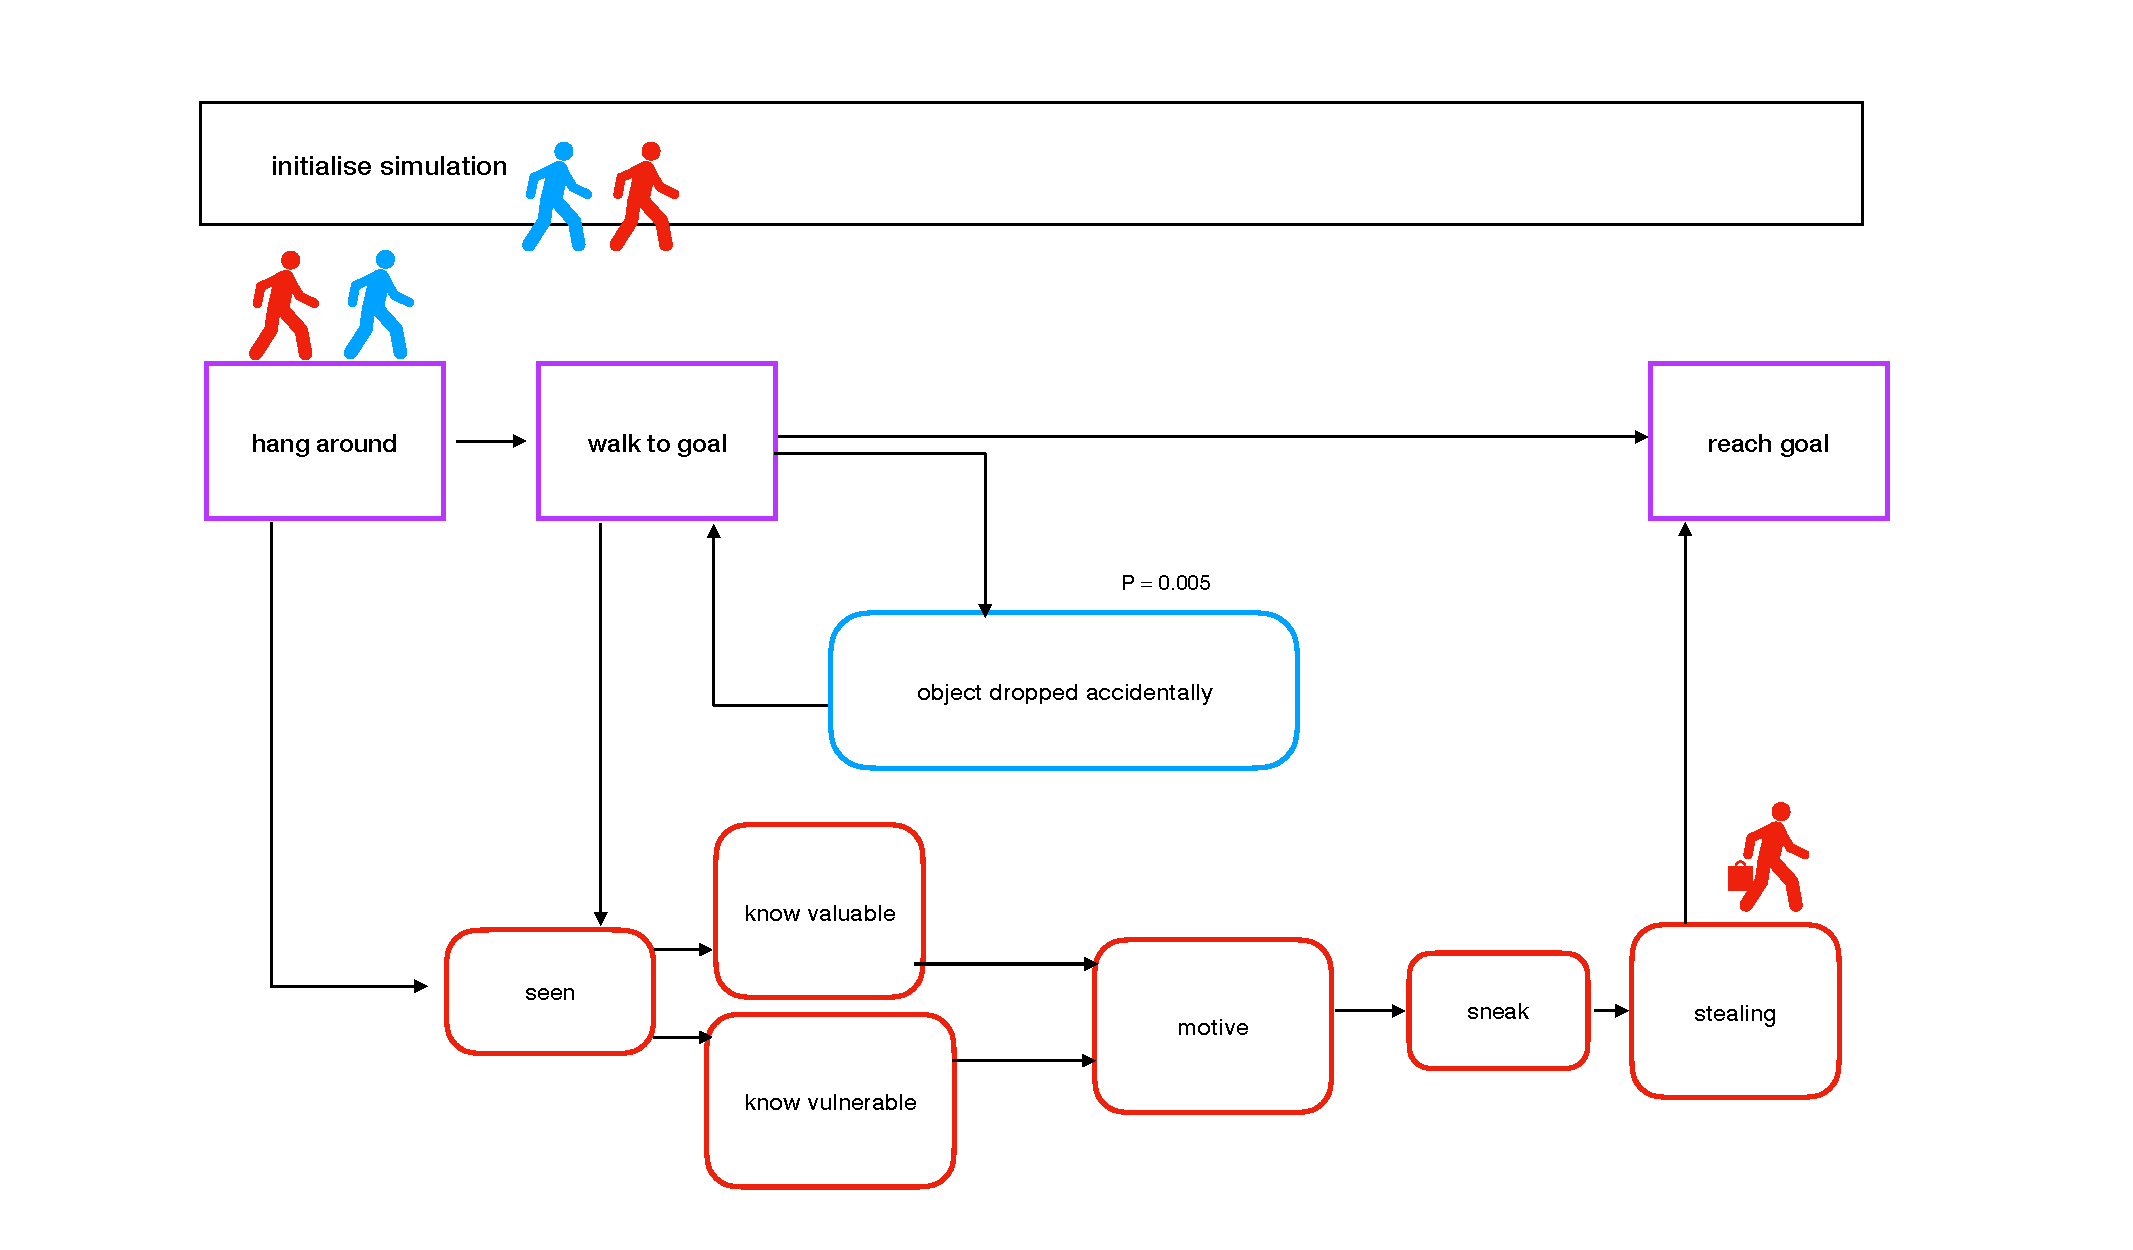
\includegraphics[width=\linewidth]{images/grotemarkt.pdf}
\end{center}
\caption{The behaviour of the agents. The nodes with rounded edges correspond to the nodes in the Bayesian Network.}
\label{behaviourGM}
\end{figure}


\begin{figure}[htbp]
\begin{center}
\begin{subfigure}{.5\textwidth}
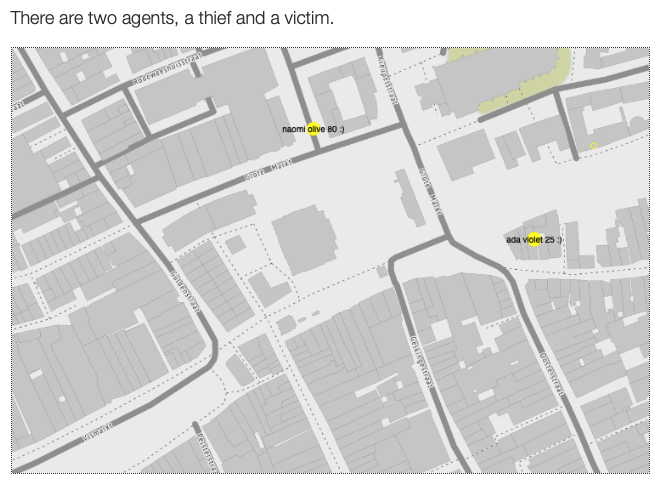
\includegraphics[width=\linewidth]{images/grotemarktmap.png}
\caption{map of environment - 2 agents}
\end{subfigure}%
\begin{subfigure}{.5\textwidth}
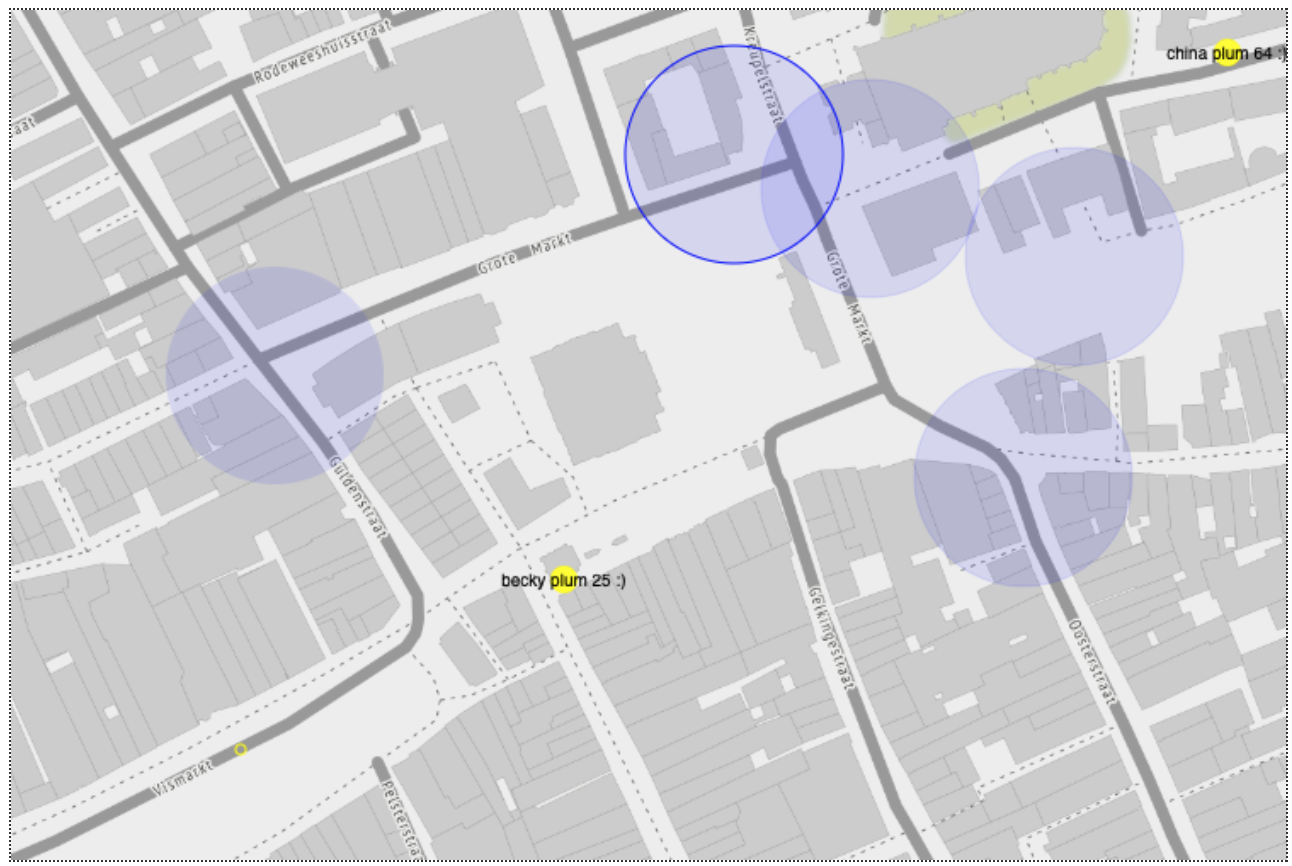
\includegraphics[width=\linewidth]{images/agentGM.png}
\caption{Camera locations are randomly initialized}
\end{subfigure}%
\caption{The Grote Markt environment}
\label{groteMarkt}
\end{center}
\end{figure}



Every simulation was run for 100 steps, or until both agents were in their target states. To find the limiting frequencies of events in the simulation, the simulation was run 10,000 times. BNs were created and evaluated based on different number of runs, to evaluate how the accuracy of the BN depends on the data available to it. The different number of runs of the simulation were [1, 5, 10, 20, 40, 60, 100, 200, 500, 1000~] for creating the BNs.



\subsection{Automatically building the network}

The output of this method is the collection of runs $O$, where each run is the global state $G$ of the simulation, as measured by the random variables $R$. These random variables become the nodes in the Bayesian Network.

The Bayesian Network is generated automatically, using the automated BN learner method as implemented in pyAgrum. There are several learners implemented in pyAgrum.\footnote{An introduction to structure learning using PyAgrum: \url{http://webia.lip6.fr/~phw/aGrUM/docs/last/notebooks/structuralLearning.ipynb.html}} The algorithm used in this experiment to structure the Bayesian Network from the simulation data is the K2 algorithm \citep{Cooper1992}. 

The K2 algorithm is a greedy search algorithm that attempts to maximise the posterior probability of the network by correctly connecting parent nodes to child nodes. It takes an ordering on the nodes as input. The first node in the ordering $X_0$ does not have any parents. For two nodes $X_i$ and $X_j$, $X_j$ cannot be the parent node of $X_i$ if $j > i$: a node can only have a parent that is earlier in the ordering. The algorithm processes each node $X_i$ by adding possible parent nodes to $X_i$ (as constrained by the ordering), and maximising the score of the network. The algorithm stops if there are no parents to add, no parents improve the score, or the node has reached the maximal number of parents \citep{Chen2008}.

Due to this ordering constraint, the K2 algorithm is efficient. However, finding the ordering of the nodes as input for the network is not trivial. The ordering should be meaningful, to reflect causal or temporal information present in the domain. By adding the nodes to the simulation in the relevant order, we can ensure that the order is temporal. The useful temporal ordering as presented to the algorithm is the the same order as the RVs are described throughout this paper. 

\subsection{Evaluating the network}

We can evaluate the response of the Bayesian Network using the effect of cumulative evidence on the posterior probability of the output nodes. This means that we order the evidence nodes chronologically, then instantiate every evidence node to a truth value (either T or F) in order. Then, we measure the posterior probability of all output nodes. This results in a diagram or table where we can see the evidence strength of each piece of true or false evidence reflected. We propose a method for evaluating Bayesian Networks over all possible global evidence states in this paper. This method is described here.

\begin{enumerate}
\item Select all evidence nodes (a total of $e$ states).
\item Order the evidence nodes chronologically.
\item Select all possible evidence states. An evidence state is a valuation of evidence, where for every evidence node, a truth value is specified. For this simulation, an evidence state could look like (1, 0, 0, 1), which would correspond to finding that the psychological report is true, the agent was seen on camera, but not seen stealing, and the object was lost.

If there is enough data available, as is the case in our simulation, we can extract these automatically. If we do not have enough data, we need to manually consider each evidence state (start with $2^e$ states, ask an elicitor to delete states that are not possible).
\item For each possible evidence state, create a total probability distribution over all possible output states. Speaking generically about two alternative, non-mutually exclusive outcomes scenario 1 (scn1) and scenario 2 (scn2), we need to find a probability distribution over $scn1, \neg scn1 \land scn2, \neg scn1 \land \neg scn2$ that is constrained by $P(scn1) + P(\neg scn1 \land scn2) + P(\neg scn1 \land \neg scn2) = 1$. Or, a weaker version, we create a preference ordering on $scn1, \neg scn1 \land scn2, \neg scn1 \land \neg scn2$, without specifying probabilities. 

In our simulation, or in data-rich environments, we can automatically create this total probability distribution, since we can count the conditional frequencies that occur in simulation. In real life, a preference ordering or probability distribution over the possible outcomes would need to be elicited by modellers from experts.
\item Create a BN.
\item For every possible evidence state, turn the relevant nodes in the BN on in order. At each step, record the posterior probability over the output nodes. Automatically convert the probability distribution over the outcomes into a preference ordering.
\item Compare the BN prediction of output nodes given evidence to the prediction establishes in step 4). Once all evidence is added, we can calculate the divergence of the BN prediction and the actual frequency in the simulation by \[|P(output|E) - F(output|E)|\], where $E$ is the total set of evidence in a given state.
\item Calculate the total accuracy per output node by \[\frac{\sum_{i=0}^{e}|P(output | E_i) - F(output| E_i)|}{e}\] For the preference ordering, we do the same, only we calculate a counting score: when the preference ordering extracted from the BN is the same as the one from the simulation, we give a point, otherwise we do not, then average this over all sets of evidence.
\end{enumerate}


\section{Results}



We have a final Bayesian Network (Figure~\ref{bullet}), that was created from the K2 algorithm that contains all the nodes specified. The arcs between nodes are not causal but conditional. We have a plot of the overall accuracy over all evidence sets of the network for both the `stealing\_1\_0' node and the `object\_dropped\_accidentally\_0' node (Figure~\ref{girl}). For a low number of runs, the network could not be created, hence the accuracy of 0. At around 10 runs, a network could be created, with an accuracy on all cumulative evidence states of around 0.75 for both nodes. Increasing the number of runs, hence, the data available to K2 to create the network, results in a higher accuracy. We have a frequency distribution over the possible states (Figure~\ref{fifteen}), where we see that most possible states occur infrequently, while one possible state [0, 1, 0, 0] occurs 70\% of the time. 

In Figures~\ref{nobody}, ~\ref{whirl}, we show cumulative evidence plots on both output nodes for two sets of evidence, on both a BN that was created from 10 runs, and on a BN that was created from 1000 runs of the simulation. Every plot shows the BN predicted output (bar on the left side), next to the actual frequencies in the simulation (bar on the right side).

In Tables~\ref{journal}, \ref{somebody}, we show the final cumulative probability and preference ordering for the output nodes as the worst (10 runs) and best (1000 runs) BN predicted them. In Table~\ref{heretic}, we show the frequency of the output for each possible evidence state, as well as the preference ordering, for the ground truth as found in the simulation.




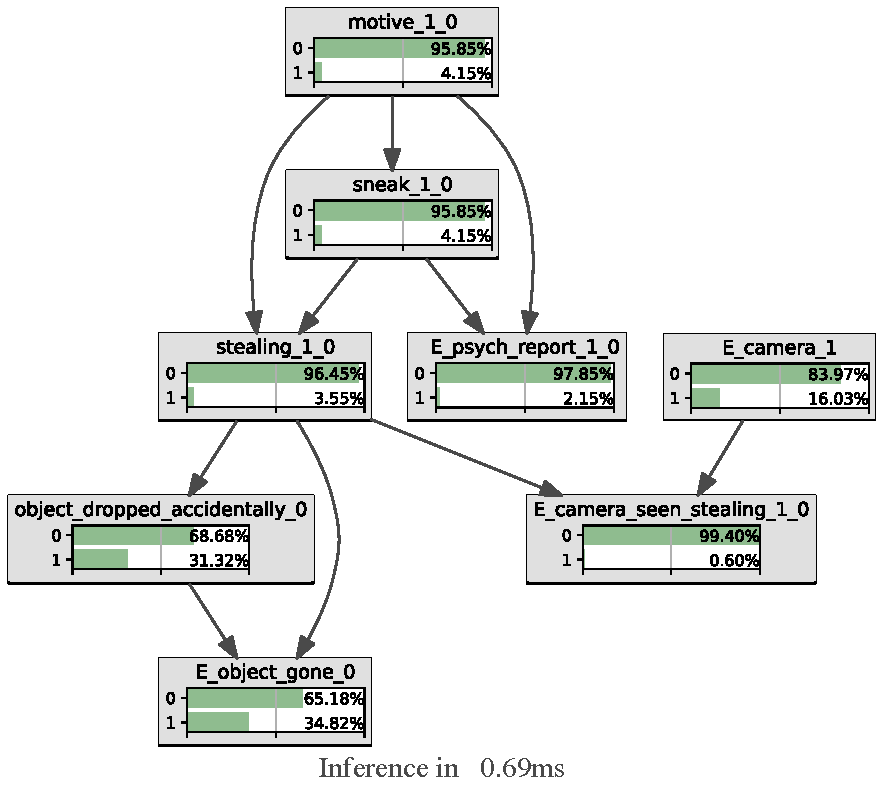
\includegraphics[]{../images/BNIMAGEGroteMarktPrivate.pdf}


\begin{figure}[htbp]
\begin{center}
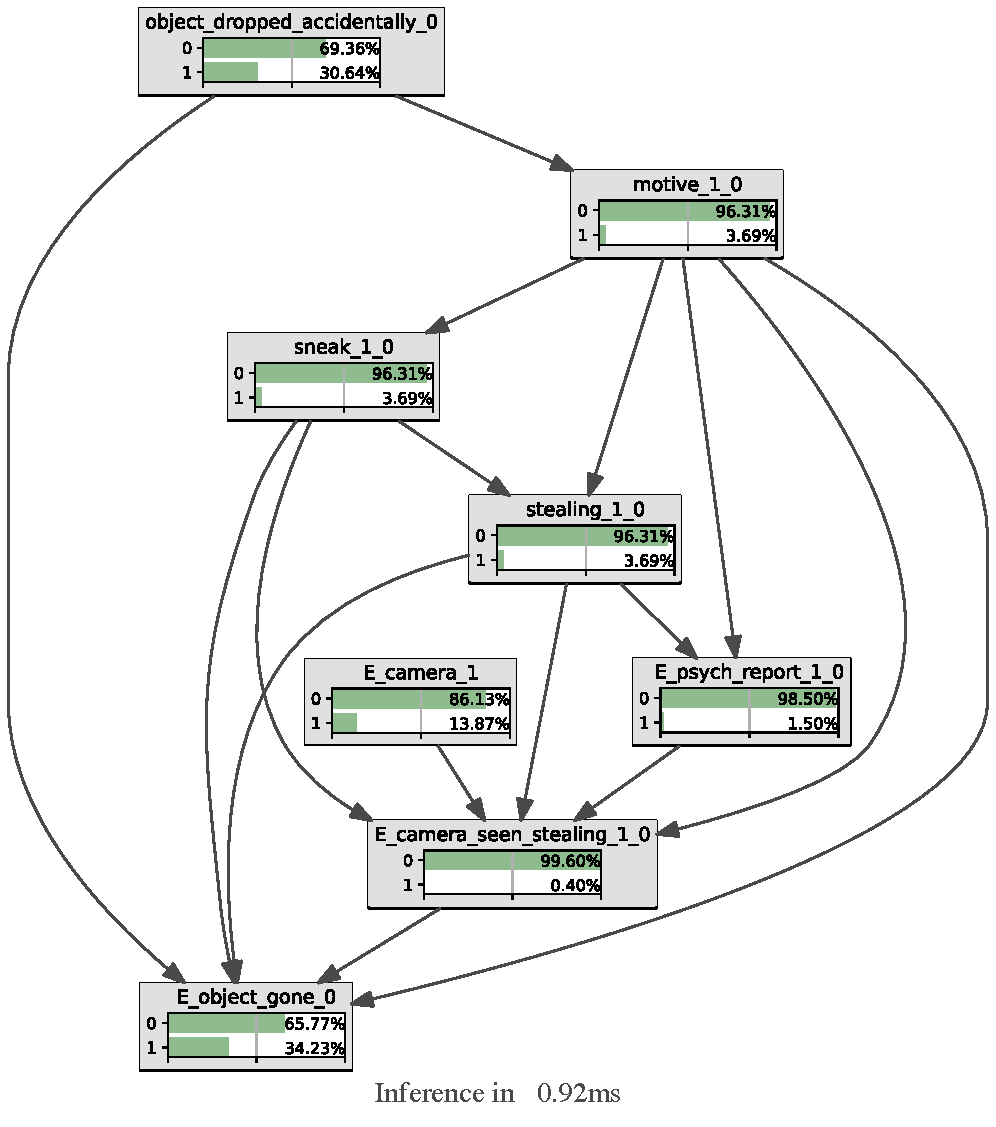
\includegraphics[width=\linewidth]{../../../experiments/GroteMarktPrivate/bnImage/BNIMAGEGroteMarktPrivate.pdf}
\caption{The final network (1000 runs)}
\label{bullet}
\end{center}
\end{figure}

\begin{figure}[htbp]
\begin{center}
\begin{subfigure}{0.6\textwidth}
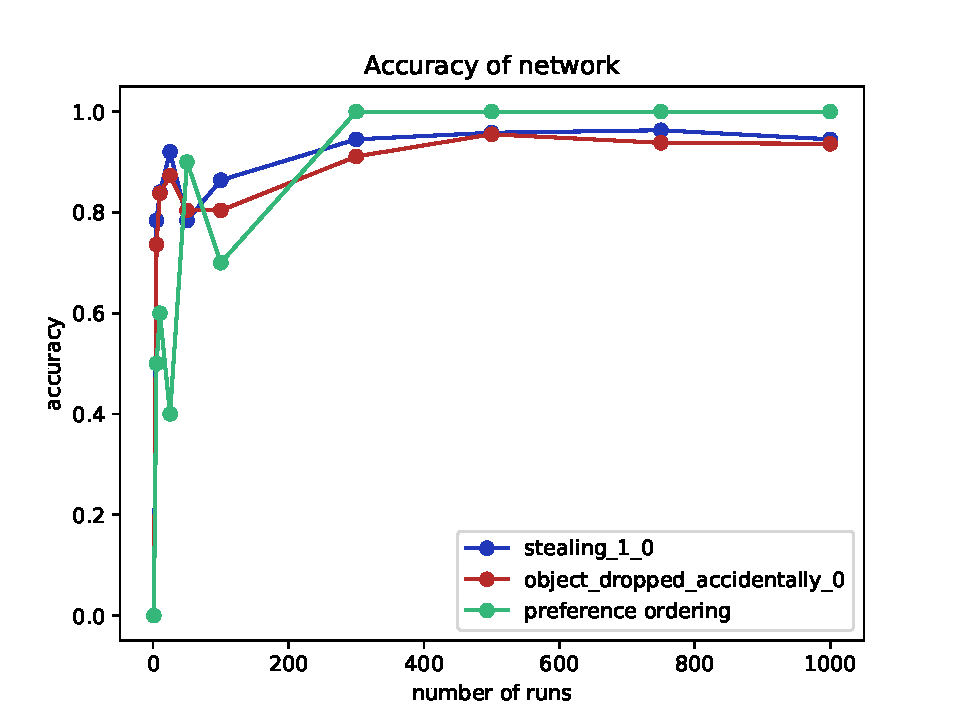
\includegraphics[width=\linewidth]{../../../experiments/GroteMarktPrivate/plots/accuracy.pdf}
\caption{Accuracy of network based on the number of training runs}
\label{girl}
\end{subfigure}%
\begin{subfigure}{0.6\textwidth}
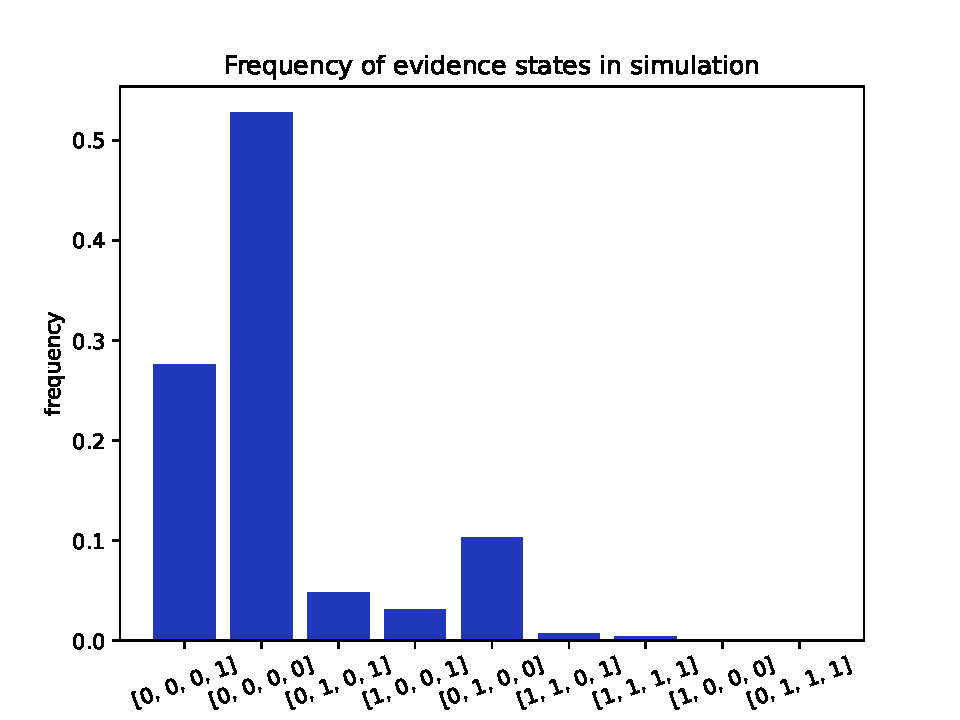
\includegraphics[width=\linewidth]{../../../experiments/GroteMarktPrivate/plots/freqStates.pdf}
\caption{Frequency of states}
\label{fifteen}
\end{subfigure}
\end{center}
\end{figure}


\begin{figure}[htbp]
\begin{center}
\begin{subfigure}{\textwidth}
\makebox[\textwidth][c]{
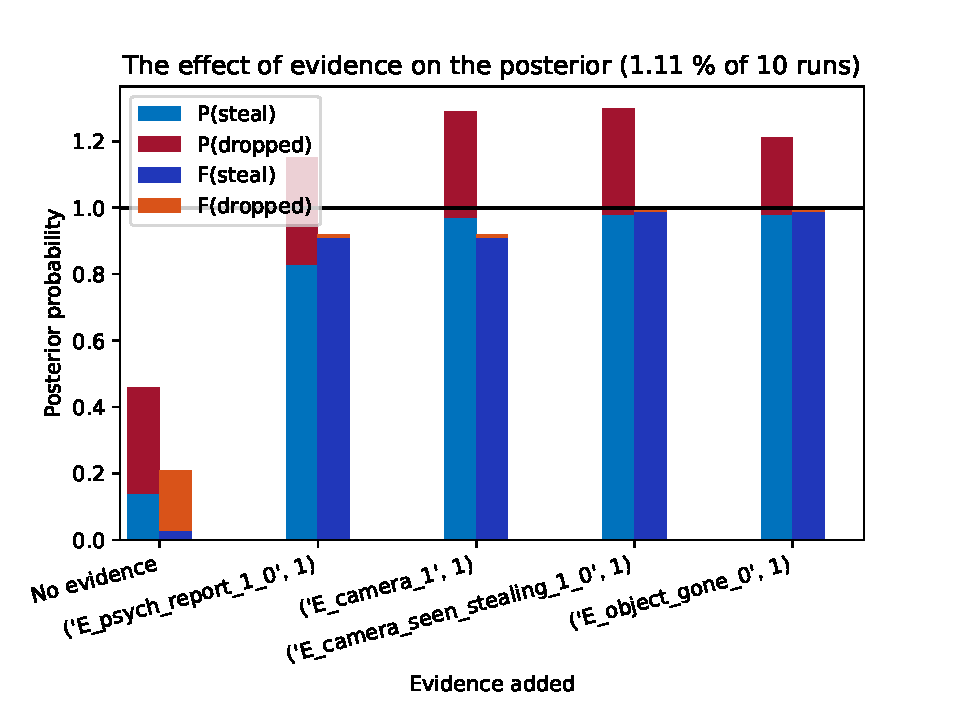
\includegraphics[width=0.7\textwidth]{../../../experiments/GroteMarktPrivate/plots/freq/evidence_progress_GroteMarktPrivate_10_1.1100.pdf}
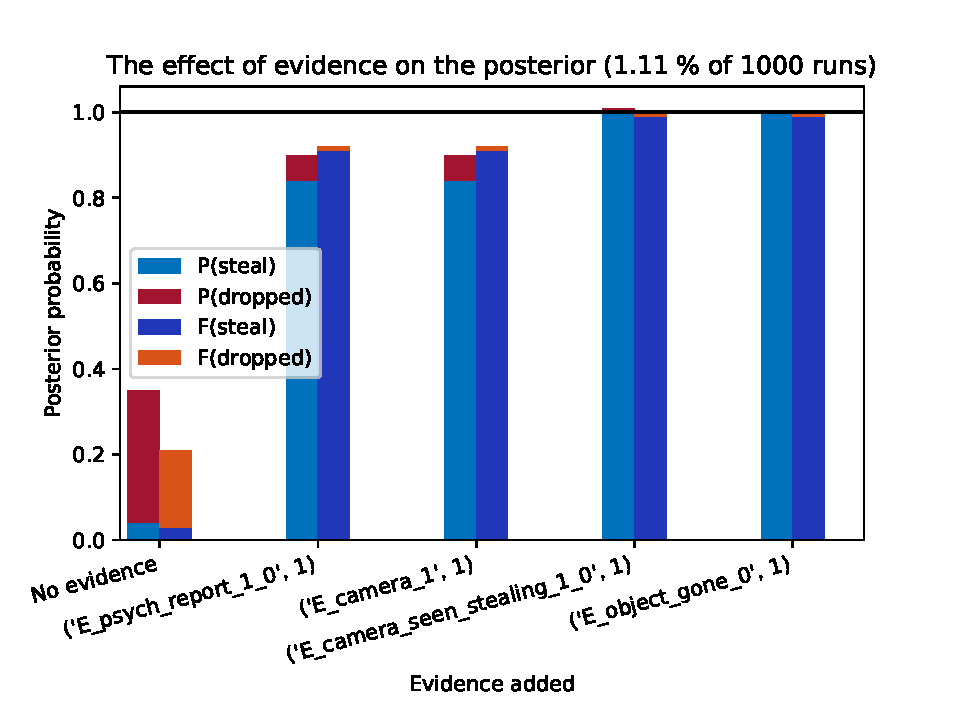
\includegraphics[width=0.7\textwidth]{../../../experiments/GroteMarktPrivate/plots/freq/evidence_progress_GroteMarktPrivate_1000_1.1100.pdf}}
\caption{Cumulative evidence on the most relevant state on 10 and 1000 runs}
\label{nobody}
\end{subfigure}

\begin{subfigure}{\textwidth}
\makebox[\textwidth][c]{
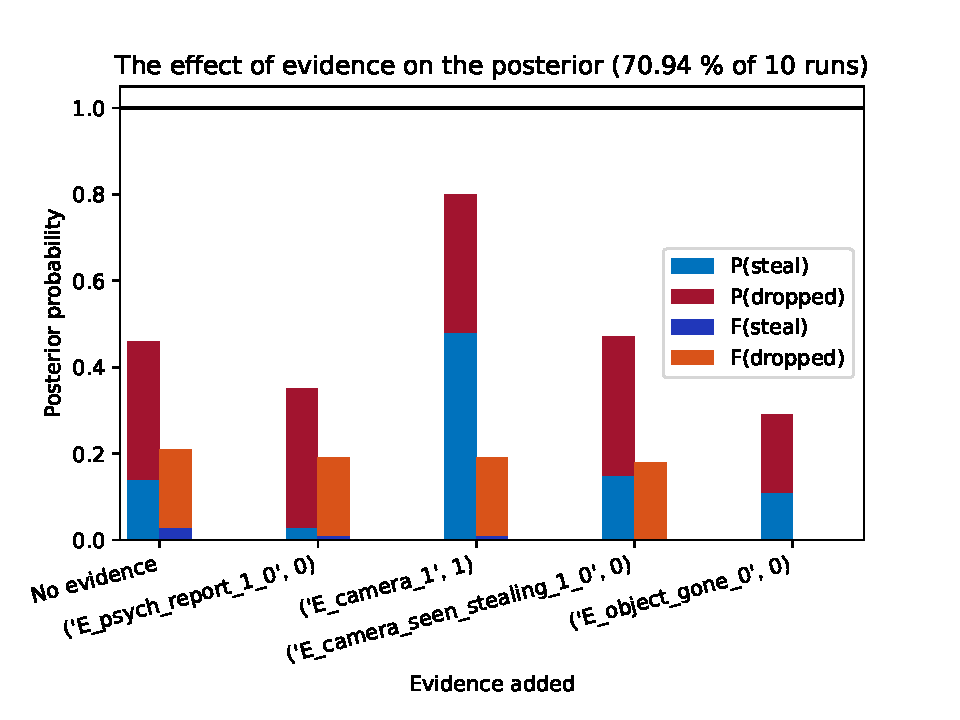
\includegraphics[width=0.7\textwidth]{../../../experiments/GroteMarktPrivate/plots/freq/evidence_progress_GroteMarktPrivate_10_70.9400.pdf}
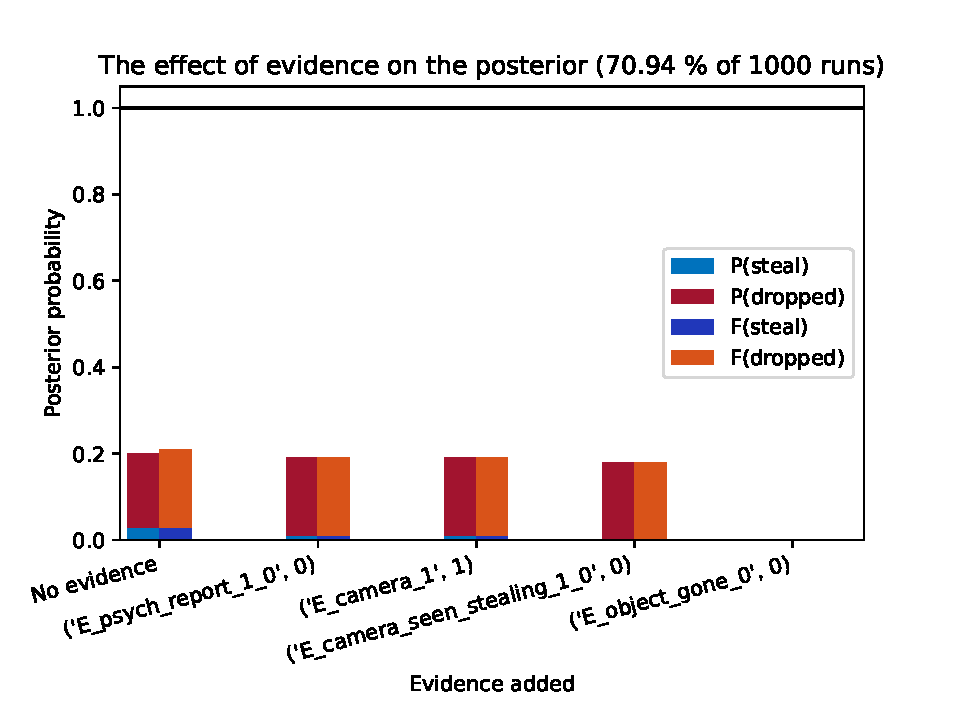
\includegraphics[width=0.7\textwidth]{../../../experiments/GroteMarktPrivate/plots/freq/evidence_progress_GroteMarktPrivate_1000_70.9400.pdf}}
\caption{Cumulative evidence on the most frequent state on 10 and 1000 runs }
\label{whirl}
\end{subfigure}
\end{center}
\end{figure}


\begin{table}
\begin{center}
\begin{tabular}{|l|c|c|c|}
\hline
evidence & H1 & H2 & H3 \\
\hline
(0, 1, 0, 0)&P(neither) (0.97) & P(dropped) (0.02) & P(steal) (0.01) \\
(0, 1, 0, 1)&P(dropped) (0.96) & P(neither) (0.03) & P(steal) (0.01) \\
(0, 0, 0, 0)&P(neither) (0.97) & P(dropped) (0.02) & P(steal) (0.01) \\
(0, 0, 0, 1)&P(dropped) (0.96) & P(neither) (0.03) & P(steal) (0.01) \\
(0, 1, 1, 1)&P(dropped) (0.96) & P(steal) (0.12) & P(neither) (-0.08) \\
(1, 1, 1, 1)&P(steal) (0.96) & P(dropped) (0.21) & P(neither) (-0.17) \\
(1, 0, 0, 1)&P(steal) (0.59) & P(dropped) (0.21) & P(neither) (0.20) \\
(1, 1, 0, 1)&P(steal) (0.59) & P(dropped) (0.21) & P(neither) (0.20) \\
(0, 1, 1, 0)&P(neither) (0.86) & P(steal) (0.12) & P(dropped) (0.02) \\
(1, 1, 0, 0)&P(dropped) (0.70) & P(steal) (0.59) & P(neither) (-0.29) \\
\hline
\end{tabular}
\end{center}
\caption{ Low number of runs, probability estimates for all cumulative evidence sets for runs =  10}
\label{journal}
\end{table}

\begin{table}[htbp]
\begin{center}
\begin{tabular}{|l|c|c|c|}
\hline
evidence & H1 & H2 & H3 \\
\hline
(0, 1, 0, 0)&P(neither) (1.00) & P(steal) (0.00) & P(dropped) (0.00) \\
(0, 1, 0, 1)&P(dropped) (0.99) & P(steal) (0.01) & P(neither) (0.00) \\
(0, 0, 0, 0)&P(neither) (1.00) & P(steal) (0.00) & P(dropped) (0.00) \\
(0, 0, 0, 1)&P(dropped) (0.95) & P(steal) (0.05) & P(neither) (0.00) \\
(0, 1, 1, 1)&P(steal) (1.00) & P(dropped) (0.01) & P(neither) (-0.01) \\
(1, 1, 1, 1)&P(steal) (1.00) & P(dropped) (0.00) & P(neither) (0.00) \\
(1, 0, 0, 1)&P(steal) (1.00) & P(dropped) (0.01) & P(neither) (-0.01) \\
(1, 1, 0, 1)&P(steal) (0.98) & P(dropped) (0.02) & P(neither) (0.00) \\
(0, 1, 1, 0)&P(steal) (0.41) & P(neither) (0.37) & P(dropped) (0.22) \\
(1, 1, 0, 0)&P(neither) (0.97) & P(steal) (0.02) & P(dropped) (0.01) \\
\hline
\end{tabular}
\end{center}
\caption{ Preference ordering with numbers on Bayesian Network prediction for all evidence states (runs 1000)}
\label{somebody}
\end{table}
\begin{table}[htbp]
\begin{center}
\begin{tabular}{|l|c|c|c|}
\hline
evidence & H1 & H2 & H3 \\
\hline
(0, 1, 0, 0)&F(neither) (1.00) & F(steal) (0.00) & F(dropped) (0.00) \\
(0, 1, 0, 1)&F(dropped) (0.98) & F(steal) (0.02) & F(neither) (0.00) \\
(0, 0, 0, 0)&F(neither) (1.00) & F(steal) (0.00) & F(dropped) (0.00) \\
(0, 0, 0, 1)&F(dropped) (0.94) & F(steal) (0.06) & F(neither) (0.00) \\
(0, 1, 1, 1)&F(steal) (0.95) & F(dropped) (0.05) & F(neither) (0.00) \\
(1, 1, 1, 1)&F(steal) (0.99) & F(dropped) (0.01) & F(neither) (0.00) \\
(1, 0, 0, 1)&F(steal) (1.00) & F(dropped) (0.00) & F(neither) (0.00) \\
(1, 1, 0, 1)&F(steal) (1.00) & F(dropped) (0.00) & F(neither) (0.00) \\
(0, 1, 1, 0)&F(neither) (1.00) & F(steal) (0.00) & F(dropped) (0.00) \\
(1, 1, 0, 0)&F(neither) (1.00) & F(steal) (0.00) & F(dropped) (0.00) \\
\hline
\end{tabular}
\end{center}
\caption{ Preference ordering with numbers for all evidence states on `ground truth' for runs=10000}
\label{heretic}
\end{table}




\section{Discussion}
In this section we discuss the success of the method, its generalisability, and future research.


\subsection{Can we use testing over all possible cumulative evidence as a way to evaluate Bayesian Networks?}
With this method, we can show that we can create BNs that predict output probabilities that correspond to the limiting frequencies of events in the simulation. We see that both the preference ordering as well as the probabilities in the output nodes in Table~\ref{somebody} are near identical to those in Table~\ref{heretic}. This means that the best BN reflects the frequencies in the simulation well, not just on one set of cumulative evidence, but on nearly all sets of cumulative evidence. 

The only evidence set where the BN does not reflect the ground truth, is for the evidence set of (0, 1, 1, 0). This is a situation where the agent is seen stealing, but the object is not gone. In the test data of 10,000 entries, there is never an entry where both stealing and dropping are true. Hence, we find that the BN does not predict the output correctly in this case. 

When less data is available to the K2 algorithm, such as the case where the simulation was run for 10 times (Table~\ref{journal}), we find that the accuracy of the network decreases. This means that the network is less able to predict the right outcome across all possible evidence states.

This method also allows us to see when the BN is assigning probability values to mutually exclusive nodes that violate probabilistic constraints. The joint probability over all three states (steal, drop, neither) can never be greater than 1, which means that none of the probability values of steal, drop, and neither, can be smaller than 0. However, in both Table~\ref{journal}, and Table~\ref{somebody}, we find that P(`neither') can sometimes be smaller than 0. This is also visible in the cumulative probability plots (see Figure~\ref{nobody} where for E\_camera\_seen\_stealing\_1\_0, the joint probability of outcomes $>$ 1). This shows that the mutually exclusive relation between stealing and dropping is not learned correctly in the network. This improves (but is not gone), when the K2 algorithm has access to more data.


This method of evaluating a BN over all states of cumulative evidence can distinguish between better and worse BNs, shows when a BN goes wrong and gives us insight in why that happens. Modellers of data-poor BNs are might think about creating an expected preference ordering on all possible evidence states, before starting to build and test the BN, in order to check whether their BN aligns with their common-sense predictions. If the BN is wrong, this is a sign that either the modeller's estimation is wrong, or that the probabilities as entered in the BN are not correctly representing your actual beliefs.


\subsection{Limitations of this approach - Plausibility of generalisability}

There are three main problems with this approach that limit its generalisability. These problems are the combinatorial explosion of the evidence states, the implausibilities of finding proper grounding, and the imprecision of the BN definitions of the random variables in real life.

\begin{enumerate}

\item For this approach, we need to consider all possible evidence states. In the worst case, if we have $e$ evidence states, this means that we have $e^2$ possible evidence states. We would have to define a preference ordering or probability distribution on the output nodes in $2^e$ cases. While this is plausible in a network with only 4 evidence nodes like this one, this becomes implausible for a case like the Anjum case study in \citet{vlek2016}, with 20 nodes ($2^20$), or \citet{Fenton2019}, with $2^13$ states. Even determining which states are not possible, is improbable with this constraint. This is a combinatorial explosion, where you would need to define many more cases of evidence than you are actually reasoning with. However, we are already doing this implicitly by using a Bayesian Network for reasoning in the first place. 

\item Due to the simulation approach in this paper, we can establish a statistical ground truth in step 4) of our method. We can create both a joint probability distribution and a preference ordering automatically from the simulation. In real life, this would have to be elicited in some way. Even if we assume that we are not in a combinatorial explosion, we would still need to define either a subjective probability distribution over all possible outcomes, or a preference ordering, and use this as a baseline to test the predictions of our BN against. This involves subjectivity twice: first in defining the preference ordering or probability distribution over outcomes, and second the probabilities that are inputted in the CPTs. Future research might establish how successful people are in estimating preference orderings or probability distributions over output nodes, so that we can use these subjective orderings as a baseline, instead of an ordering generated by frequency data from the simulation.

\item More generally, a problem with BNs is that a random variable, which is a function that maps a set of events to a `measurable space'. Informally, in this case, the RV maps an event to either T or F. There are two problems: how we define the set of events that we are mapping (domain), and the validity of the `mapping' function.

\begin{enumerate}
\item \textbf{Defining the domain, or the reference class problem:} Defining the set of events is inherently problematic, and is called `the problem of the reference class' \citep{colyvan2001}. The problem of the reference class is in picking the set of events that belong in the domain. This problem is relevant in both the simulation and the real world.  However it is not as relevant in the simulation because often there is only one interesting/relevant way to interpret the events (eg there are not two equally ``good'' `reference classes' for a node like `sneak\_1\_0'). There is only one relevant class (which is defined with respect to the agent behaviour), and that is the relevant reference class. However, in real life, you cannot know which reference class is the most `relevant' or fair to choose. It is unclear how to get out of this bind, but we know that we do reason pragmatically and informally with the reference class.
\item \textbf{Defining the mapping, and its validity:} This is no problem in the simulation, we know what the methods for determining the probabilities in the nodes are valid (which means that they always correctly reflect the underlying progress that is generating them), because it's literally programmed in this way - directly reflecting the states, we literally just count the frequencies. However, in real life, we might not even know the validity of different possible mappings for the same node. In short, how do we determine in real life that `sneak\_1\_0'? How can we determine if anyone is actually `sneaking', and how will we know if this method of determination is valid? This is also why BNs for forensic-statistical BNs are more legitimate: in these forensic-statistic fields, we have defined clear methods and we know the method through which we are mapping: these variables are operationalised. This is not the case for more `vague' nodes.
\end{enumerate}
\end{enumerate}

 
\subsubsection{Future Research}

The simulation in this paper is not complex, and does not model reality in any realistic way. The purpose of this simulation was just to generate data, and did not need to reflect any specific facts about the world. However, agent-based modelling can be useful for investigating different aspects of Bayesian Networks, or reasoning with evidence more generally. Increasing the level of the simulation from level 0 to something that reflects reality is useful to investigate problems such as the Opportunity Prior as presented in \citet{Fenton2017}. 


 
\subsubsection{Future Research}

The simulation in this paper is not complex, and does not model reality in any realistic way. The purpose of this simulation was just to generate data, and did not need to reflect any specific facts about the world. However, agent-based modelling can be useful for investigating different aspects of Bayesian Networks, or reasoning with evidence more generally. Increasing the level of the simulation from level 0 to something that reflects reality is useful to investigate problems such as the Opportunity Prior as presented in \citet{Fenton2017}. 


\bibliographystyle{apalike}
\bibliography{masterThesisCitations}